\begin{frame}
	\myheading{Module 19.7: Motivation for Sampling }
\end{frame}
		
\begin{frame}
	\begin{columns}
		\column{0.4\textwidth}
		\begin{overlayarea}{\textwidth}{\textheight}
			\begin{align*}
				\hspace{-0.5cm}\frac{\partial \mathscr{L}(\theta)}{\partial w_{ij}} = \mathbb{E}_{p(H|V)} [v_i h_j] - \mathbb{E}_{p(V,H)} [v_i h_j]
			\end{align*}
		\end{overlayarea}
		\column{0.6\textwidth}
		\begin{overlayarea}{\textwidth}{\textheight}
			\begin{itemize}
				\item<1-> The trick is to approximate the sum by using a few samples instead of an exponential number of samples
				\item<2-> We will try to understand this with the help of an analogy
			\end{itemize}
		\end{overlayarea}
	\end{columns}
\end{frame}



\begin{frame}
	\begin{columns}
		\column{0.45\textwidth}
		\begin{overlayarea}{\textwidth}{\textheight}
			\begin{itemize}
				\item<1-> Suppose you live in a city which has a population of 10M and you want to compute the average weight of this population
				\item<2->You can think of $X$ as a random variable which denotes a person
				\item<3-> The value assigned to this random variable can be any person from your population
				\item<4-> For each person you have an associated value denoted by $weight(X)$
				\item<5-> You are then interested in computing the expected value of $weight(X)$ as shown on the RHS
			\end{itemize}
		\end{overlayarea}
		\column{0.6\textwidth}
		\begin{overlayarea}{\textwidth}{\textheight}
			\vspace{-0.2cm}
			\onslide<6->{\begin{align*}
				\mathbb{E}[weight(X)] = \sum_{(x\in P)} p(x) weight(x)
			\end{align*}}
			\vspace{-0.6cm}
			\begin{itemize}
				\item<7-> Of course, it is going to be hard to get the weights of every person in the population and hence in practice we approximate the above sum by sampling only few subjects from the population (say 10000)
				\vspace{-0.2cm}
				\onslide<8->{\begin{align*}
					\hspace{-0.5cm}\mathbb{E}[weight(X)] \approx \frac{\sum_{x\in P[:10000]} [p(x) weight(x)]}{\sum_{x\in P[:10000]} p(x)}
				\end{align*}}
				\vspace{-0.4cm}
				\item<9-> Further, you assume that $P(X) = \frac{1}{N} = \frac{1}{10K}$, i.e., every person in your population is equally likely
				\vspace{-0.2cm}
				\onslide<10->{\begin{align*}
					\hspace{-0.5cm}\mathbb{E}[weight(X)] \approx \frac{\sum_{x\in Persons[:10000]} [weight(x)]} {10^4}
				\end{align*}}
				\vspace{-0.2cm}
			\end{itemize}
		\end{overlayarea}
	\end{columns}
\end{frame}


\begin{frame}
	\begin{columns}
	\column{0.4\textwidth}
		\begin{overlayarea}{\textwidth}{\textheight}
			\begin{align*}
				\mathbb{E}[X] = \sum_{(x\in P)} x p(x)
			\end{align*}
		\end{overlayarea}
	\column{0.6\textwidth}
		\begin{overlayarea}{\textwidth}{\textheight}
			\begin{itemize}
				\item<1-> This looks easy, why can't we do the same for our task ?
				\item<2-> Why can't we simply approximate the sum by using some samples?
				\item<3-> What does that mean? It means that instead of considering all possible values of $\{v, h\} \in 2^{m+n}$ let us just consider some samples from this population
				\item<4-> Analogy: Earlier we had 10M samples in the population from which we drew $10K$ samples, now we have $2^{m+n}$ samples in the population from which we need to draw a reasonable number of samples
				\item<5-> Why is this not straightforward? Let us see!
			\end{itemize}
		\end{overlayarea}
	\end{columns}
\end{frame}

\begin{frame}
	\begin{columns}
	\column{0.4\textwidth}
		\begin{overlayarea}{\textwidth}{\textheight}
			\centering
\vspace{0.5cm}
\tikzstyle{neuronv}=[circle,minimum size=20pt,inner sep=0pt, thick, fill=orange!30, draw=red!50]
\tikzstyle{neuronh}=[circle,minimum size=20pt,inner sep=0pt, thick, fill=blue!20, draw=blue!60]
\tikzstyle{stateTransition}=[thick]
\tikzstyle{learned}=[text=black]
\begin{tikzpicture}[scale=1.9]
    % \draw ;
    \draw[rounded corners=0.5cm, draw=red!60, thick] (-0.4, -0.25) rectangle (2.5, 0.25) {};
    \draw[rounded corners=0.5cm, draw=red!60, thick] (-0.4, 1.25) rectangle (2.5, 1.75) {};

    \node (v1)[neuronv] at (0, 0) {$v_1$};
    \node (v2)[neuronv] at (0.7, 0) {$v_2$};
    \node (v3)[] at (1.4, 0) {$\cdots$};
    \node (v4)[neuronv] at (2.1, 0) {$v_m$};
    \node[below=0.5cm of v2] (v) {$V \in \{0, 1\}^m$};
    \node[learned,below=0.1cm of v1] (bv1) {$b_1$};
    \node[learned,below=0.1cm of v2] (bv2) {$b_2$};
    % \node[learned,below=0.1cm of v3, scale=0.7] (bv3) {$b_{v_3}$};
    \node[learned,below=0.1cm of v4] (bv4) {$b_m$};

    \node (h1)[neuronh] at (0, 1.5) {$h_1$};
    \node (h2)[neuronh] at (0.7, 1.5) {$h_2$};
    \node (h3)[] at (1.4, 1.5) {$\cdots$};
    \node (h4)[neuronh] at (2.1, 1.5) {$h_n$};
    \node[above=0.5cm of h2] (h) {$H \in \{0, 1\}^n$};
    \node[learned,above=0.1cm of h1] (bv1) {$c_1$};
    \node[learned,above=0.1cm of h2] (bv2) {$c_2$};
    % \node[learned,below=0.1cm of v3, scale=0.7] (bv3) {$b_{v_3}$};
    \node[learned,above=0.1cm of h4] (bv4) {$c_n$};

    \node[learned, scale=0.7] (W) at (2.5, 0.75) {$W \in \mathbb{R}^{m \times n}$};

    \draw[learned,stateTransition] (0,0.17) -- (0,1.33) node [midway,left=-0.1cm] {$w_{1,1}$};
    \draw[stateTransition] (0,0.17) -- (0.7,1.33) node [midway,above=-0.06cm,sloped] {};
    \draw[stateTransition] (0,0.17) -- (2.1,1.33) node [midway,above=-0.06cm,sloped] {};

    \draw[stateTransition] (0.7,0.17) -- (0,1.33) node [midway,above=-0.06cm,sloped] {};
    \draw[stateTransition] (0.7,0.17) -- (0.7,1.33) node [midway,above=-0.06cm,sloped] {};
    \draw[stateTransition] (0.7,0.17) -- (2.1,1.33) node [midway,above=-0.06cm,sloped] {};

    \draw[stateTransition] (2.1,0.17) -- (0,1.33) node [midway,above=-0.06cm,sloped] {};
    \draw[stateTransition] (2.1,0.17) -- (0.7,1.33) node [midway,above=-0.06cm,sloped] {};
    \draw[learned,stateTransition] (2.1,0.17) -- (2.1,1.33) node [midway,left=-0.1cm] {$w_{m,n}$};

\end{tikzpicture}
		\end{overlayarea}
	\column{0.6\textwidth}
		\begin{overlayarea}{\textwidth}{\textheight}
			\begin{itemize}
				\item<1-> For simplicity, first let us just focus on the visible variables $(V \in 2^{m})$ and let us see what it means to draw samples from $P(V)$
				\item<2-> Well, we know that $V = v_1, v_2, \ldots, v_m$ where each $v_i \in \{0,1\}$
				\item<3-> Suppose we decide to approximate the sum by $10K$ samples instead of the full $2^{m}$ samples
				\item<4-> It is easy to create these samples by assigning values to each $v_i$
				\item<5-> For example, $V = 11111\ldots 11111, V = 00000\ldots 0000, V = 00110011\ldots 00110011, \ldots V = 0101\ldots 0101$ are all samples from this population
				\item<6-> So which samples do we consider ?
			\end{itemize}
		\end{overlayarea}
	\end{columns}
\end{frame}

\begin{frame}
	\begin{columns}
		\column{0.4\textwidth}
		\begin{overlayarea}{\textwidth}{\textheight}
			\centering
			\onslide<5->{\begin{figure}
				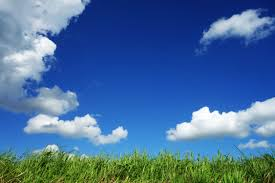
\includegraphics[width=80pt,height=60pt]{images/sunnysky}
				\caption{Likely}
			\end{figure}
			\begin{figure}
				
\includegraphics[width=80pt,height=60pt]{images/random.png}
				\caption{Unlikely}
			\end{figure}}
		\end{overlayarea}
		\column{0.6\textwidth}
		\begin{overlayarea}{\textwidth}{\textheight}
			\begin{itemize}
				\item<1-> Well, that's where the catch is!
				\item<2-> Unlike, our population analogy, here we cannot assume that every sample is equally likely
				\item<3-> Why? \onslide<4->{(Hint: consider the case that visible variables correspond to pixels from natural images)}
				\item<5-> Clearly some images are more likely than the others!
				\item<6-> Hence, we cannot assume that all samples from the population $(V \in 2^{m})$ are equally likely
			\end{itemize}
		\end{overlayarea}
	\end{columns}
\end{frame}


\begin{frame}
	\begin{columns}
		\column{0.4\textwidth}
		\begin{overlayarea}{\textwidth}{\textheight}
			\centering
			\begin{figure}
				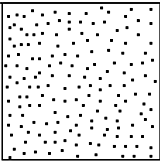
\includegraphics[scale=0.4]{images/Uniform-dist.png}
				\caption{Uniform distribution}
			\end{figure}
			\begin{figure}
				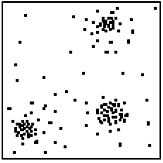
\includegraphics[scale=0.4]{images/Multimodal-dist.png}
				\caption{Multimodal distribution}
			\end{figure}
		\end{overlayarea}
		\column{0.6\textwidth}
		\begin{overlayarea}{\textwidth}{\textheight}
			\begin{itemize}
				\item<1-> Let us see this in more detail
				\item<2-> In our analogy, every person was equally likely so we could just sample people uniformly randomly
				\item<3-> However, now if we sample people uniformly randomly then we will not get the true picture of the expected value
				\item<4-> We need to draw more samples from the high probability region and fewer samples from the low probability region
				\item<5-> In other words each sample needs to be drawn in proportion to its probability and not uniformly
			\end{itemize}
		\end{overlayarea}
	\end{columns}
\end{frame}



\begin{frame}
	\begin{columns}
		\column{0.4\textwidth}
		\begin{overlayarea}{\textwidth}{\textheight}
			\begin{align*}
				\hspace{-0.5cm}\frac{\partial \mathscr{L}(\theta|V)}{\partial w_{ij}} = \mathbb{E}_{p(H|V)} [v_i h_j] - \mathbb{E}_{\color{red} p(V,H)} \color{black}[v_i h_j]
			\end{align*}
			\footnotesize{\begin{align*}
				Z=&\sum_V \sum_H \Big( \prod_i\prod_j \phi_{ij}(v_i, h_j) \\
				&\prod_i \psi_i(v_i) \prod_j \xi_j(h_j) \Big)
			\end{align*}}
		\end{overlayarea}
		\column{0.6\textwidth}
		\begin{overlayarea}{\textwidth}{\textheight}
					\begin{itemize}
				\item<1-> That is where the problem lies!
				\item<2-> To draw a sample $(V,H)$, we need to know its probability $P(V,H)$
				\item<3-> And of course, we also need this $\color{red}P(V,H)$\color{black} to compute the expectation 
				\item<4-> But, unfortunately computing $P(V,H)$ is intractable because of the partition function Z 
				% (on LHS also show the partition function Z)
				\item<5-> Hence, approximating the summation by using a few samples is not straightforward! (or rather drawing a few samples from the distribution is hard!)
			\end{itemize}
		\end{overlayarea}
	\end{columns}
\end{frame}



\begin{frame}
	\begin{block}{The story so far}
		\begin{itemize}
			\item<1-> Conclusion: Okay, I get it that drawing samples from this distribution $P$ is hard. 
			\item<2-> Question: Is it possible to draw samples from an easier distribution (say, $Q$) as long as I am sure that if I keep drawing samples from $Q$ eventually my samples will start looking as if they were drawn from $P$!
			\item<3-> Answer: Well if you can actually prove this then why not? (and that's what we do in Gibbs Sampling)
		\end{itemize}
	\end{block}
\end{frame}
